\documentclass{beamer}
\mode<presentation>
{
  \usetheme{Luebeck}
  \useoutertheme[subsection=false,footline=authortitle]{miniframes}
  \usecolortheme{dolphin}
  \usefonttheme{default}
  \setbeamertemplate{navigation symbols}{}
  \setbeamertemplate{caption}[numbered]
} 
\usepackage{pgfpages}
\setbeameroption{show notes}
\setbeameroption{show notes on second screen=right}
\setbeamertemplate{note page}[plain]

\usepackage[english]{babel}
\usepackage[utf8]{inputenc}
\usepackage{mathtools}
\usepackage{graphicx}
\graphicspath{ {graphics/} }

\title[Master's Thesis Presentation]{Can web pages be distinguished by their side channel signatures?}
\author{Emil 'Skeen' Madsen - 20105376}
\institute{Aarhus University - Computer Science}
\date{}

\begin{document}

\section*{Introduction}
\begin{frame}
  \titlepage
  
\includegraphics[scale=1]{logo}
\end{frame}

\note[itemize]{
\item Title - Also known as web page fingerprinting
\item What did we do? (short)
\begin{itemize}
\item Prove that covert channels exist in browser
\item Prove that web pages leak information
\item Prove that web pages can be distinguished \\ (web page fingerprinting)
\item Discussed practicality and defenses
\end{itemize}
}

\begin{frame}{Table of Contents}
In this presentation I will go through the two topics:
\tableofcontents
\end{frame}

\note[itemize]{
\item What I will do in this presentation
\begin{itemize}
\item Asked to present a paper \\ * Website Fingerprinting at Internet Scale
\item Relate it to our project
\end{itemize}
}

\section[Paper]{Paper - Website Fingerprinting at Internet Scale}
\begin{frame}{Main ideas}
\begin{itemize}
\item Identify web pages by encrypted and anonymized data flows
\item Computational efficiency
\item Scalability
\end{itemize}
\end{frame}

\note[itemize]{
    \item Introduce each topic of the paper briefly
    \item Tor identification has been done before
    \begin{itemize}
    \item Make it scalable (computation)
    \item How is accuracy
    \item Compares with Wang et al. (the best in literature)
    \item Larger web page sets (and more realistic ones)
    \end{itemize}
}

\begin{frame}{Encrypted data flows and anonymized data flows}
\begin{itemize}
\item What are these flows?
\item What is Tor?
\item What is the attacker model?
\end{itemize}
\end{frame}

\note[itemize]{
    \item Encrypted data flows
    \begin{itemize}
    \item TLS
    \item HTTPS
    \end{itemize}
    Only meta information such a packet sizes and direction of traffic.

    \item Encrypted and anonymized
    \begin{itemize}
    \item Tor - Most popular one \\
        Does not obscure the sizes, direction and timing of packets. \\
        Attack utilizes these metrics for fingerprinting.
    \end{itemize}

    \item Local passive eavesdropper:
    \begin{itemize}
    \item ISP
    \item Local network administrator
    \item Other customers at the cafe
    \end{itemize}
}

\begin{frame}{Experimental setup}
\begin{itemize}
\item Acquiring data sets
\begin{itemize}
\item Reference / Query set
\end{itemize}

\item Data processing
\begin{itemize}
\item Wang uses k-NN, with manually selected features.
\item Paper uses CUMUL with four data parameters:
\begin{itemize}
\item Number of incoming / outgoing packages
\item Size of incoming / outgoing packages
\end{itemize}
\end{itemize}

\item Feature extraction (resampling)
\begin{center}
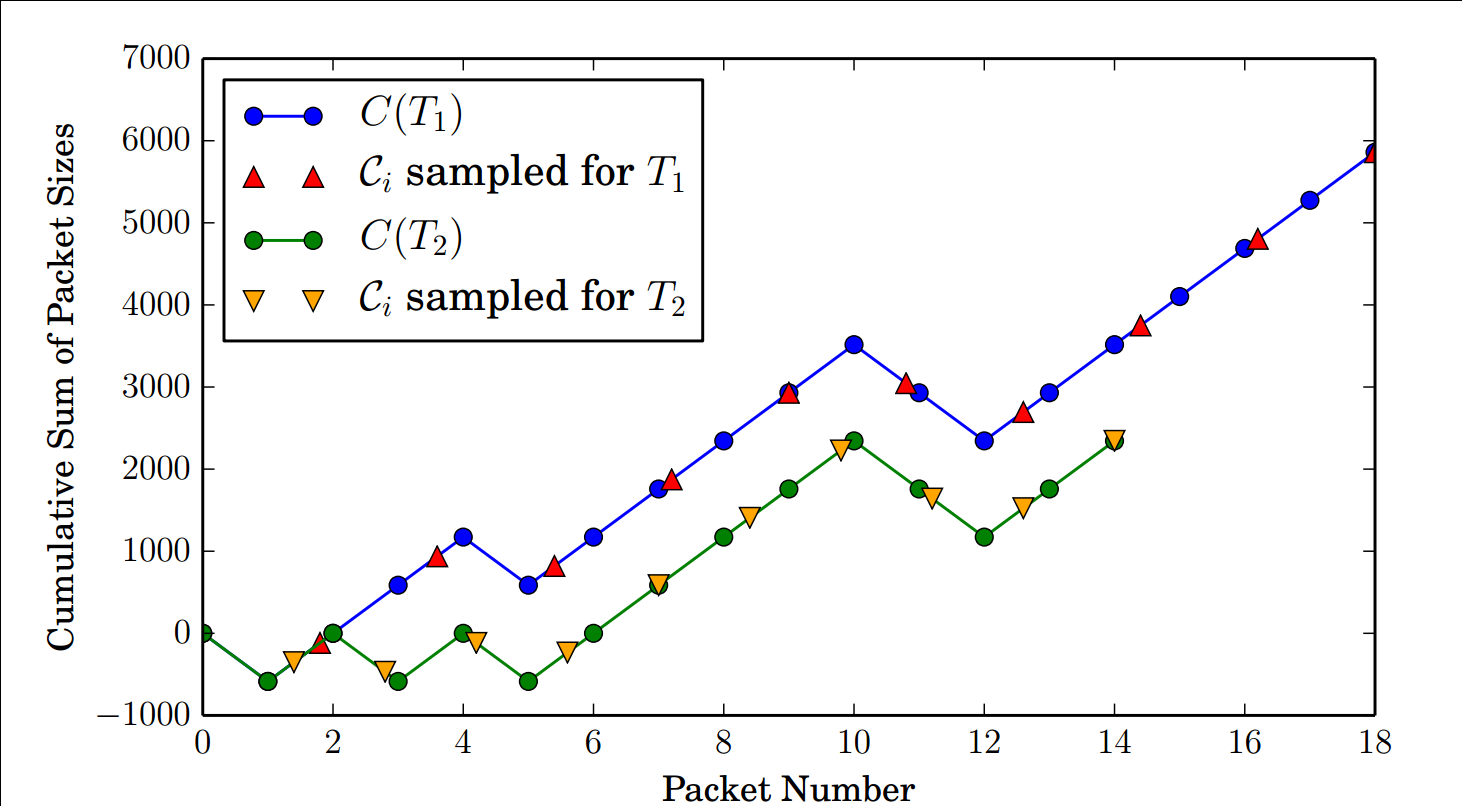
\includegraphics[width=0.5\textwidth,trim={0.1cm 0 0 0.1cm},clip]{resample}
\end{center}
Results show that $n = 100$ yields best trade-off between accuracy and computational efficiency.

\end{itemize}
\end{frame}

\note[itemize]{
    \item Reference Set - Assumed to be build by the attacker before-hand \\
        Assumed to be build in the context of the victim, creates fingerprints

    \item Query set - Recorded using tcpdump, on the local network.

    \item Wang features such as
    \begin{itemize}
    \item Unique packet lengths
    \item Concentration of outgoing packages
    \item Bursts
    \end{itemize}

    \item Paper
    \begin{itemize}
    \item Outgoing as negative
    \item Ingoing as positive
    \end{itemize}
}

\begin{frame}{Experimental proof-of-concept}
\begin{itemize}
\item Real life example, using two web pages.

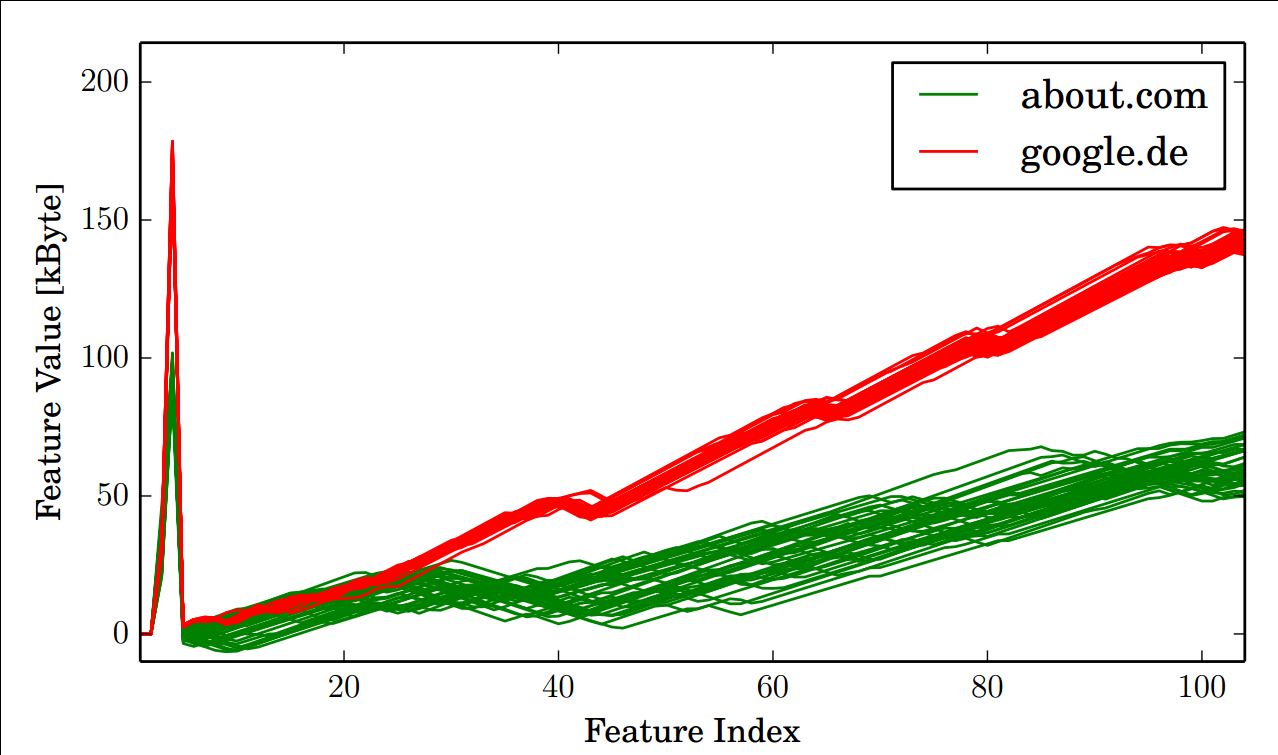
\includegraphics[width=0.8\textwidth,trim={0.1cm 0 0 0.1cm},clip]{poc}

\end{itemize}
\end{frame}

\note[itemize]{
    \item Cumulative trace of google.de versus about.com
    \item Easy visual distinction, automated using Support Vector Machines.
}

\begin{frame}{Evaluation - Setup}
\begin{itemize}
\item Open- and Closed-world tests
\item Web page evaluation sites
\item Web page vs Website vs Index page
\end{itemize}
\end{frame}

\note[itemize]{
    \item Open- and Closed-world tests
    \begin{itemize}
    \item Closed-world; All web pages are known, find accuracy. \\
        User only visits a limited number of sites.
    \item Open-world; Most web pages are unknown, reject them, and find accuracy. \\
        User can visit all sites, we filter them.
    \end{itemize}
    Argues that Alexa isn't realistic background noise (open world).

    \item Web page evaluation sites (Several, among others):
    \begin{itemize}
    \item Sets from Wang, but only for comparison
    \item 300.000 pages collected via Twitter, Google trends, ...
    \end{itemize}

    \item Web page vs Website
    \begin{itemize}
    \item Web page is a single HTML document
    \item Website is a collection of web pages
    \item Index page is the web page from a website top level.
    \end{itemize}
    Profiling web pages at scale may be infeasible, while websites are not.
}

\begin{frame}{Evaluation - Results 1 - Wang}
\begin{itemize}
\item Closed World results \\
    \begin{tabular}{lcc} \hline
                         & 90 Instances & 40 Instances \\ \hline
    k-NN (3736 features) & 90.84        & 89.19 \\
    CUMUL (104 features) & 91.38        & 92.03 \\ \hline
    \end{tabular} \newline\newline

\item Open World results \\
    \begin{tabular}{lcccc} \hline
        & \multicolumn{2}{c}{multi-class} & \multicolumn{2}{c}{two-class} \\
        & k-NN  & CUMUL & k-NN  & CUMUL \\ \hline
    TPR & 89.61 & 96.64 & 90.59 & 96.92 \\
    FPR & 10.63 & 9.61  & 2.24  & 1.98 \\ \hline
    \end{tabular}

\end{itemize}
\end{frame}

\note[itemize]{
    \item For the closed world results the attack are similar.
    \begin{itemize}
        \item The authors speculate that 90\% may be an upper limit in this case.
        \item Data may not be generalizable beyond that, doing so would yield overfitting.
        \item 100 pages with 90 / 40 instances per page.
    \end{itemize}
    \item Open world results, the attacks differ a bit more.
    \begin{itemize}
        \item 100 foreground pages (profiling) with 90 instances per page.
        \item 9000 background pages (noise) with 1 instance per page.

        \item multi-class - All foreground pages are separate classes
        \item two-class - All foreground pages are a single class

        \item multi-class has a higher rate of false positives,
            but the difference shows that most of these are between the foreground pages.

        \item two-class may be usable for seeing if a user has visited a terror,
            radicalization or otherwise blacklisted site.
    \end{itemize}
}

\begin{frame}{Evaluation - Results 2 - Wang}
\begin{itemize}
\item Performance:
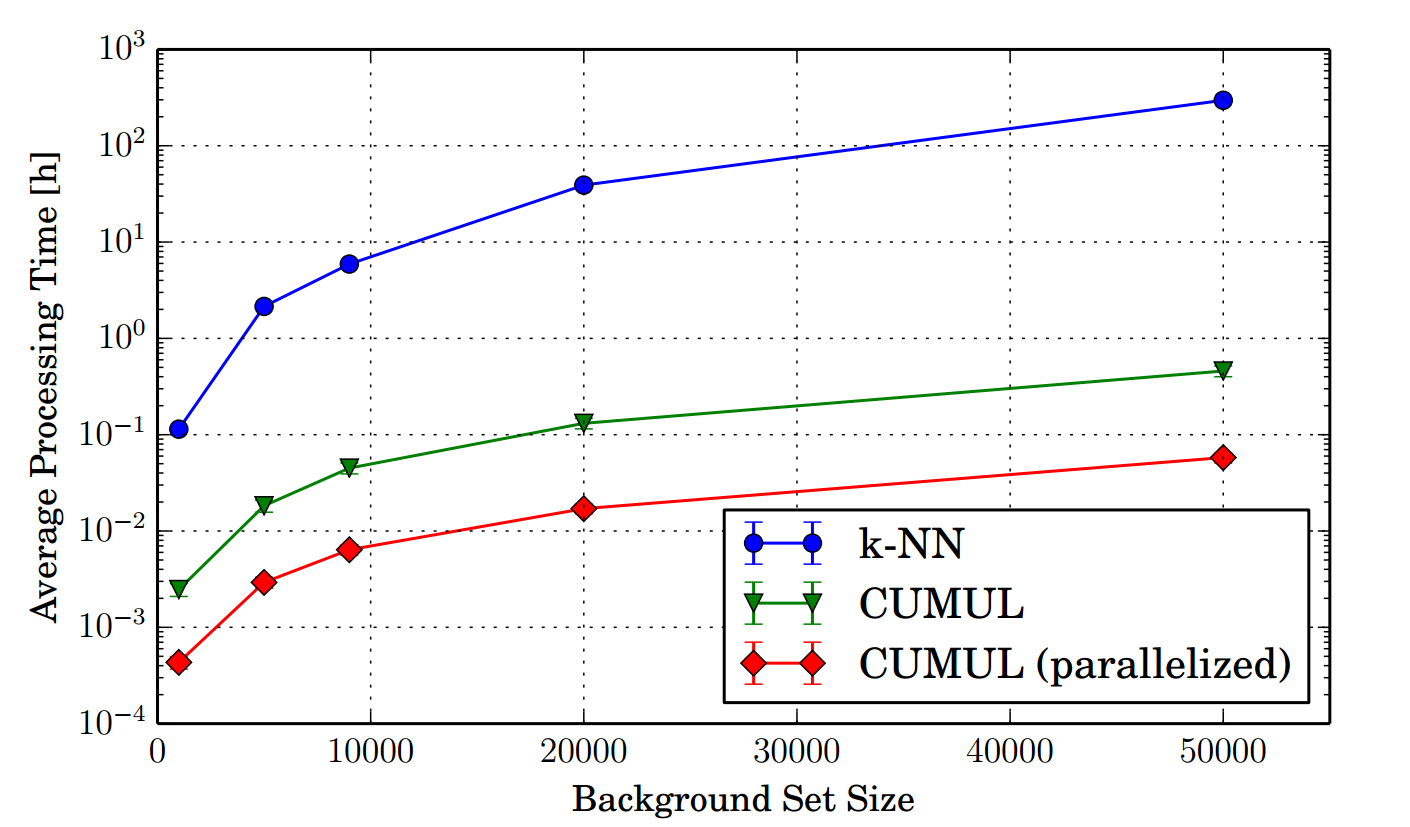
\includegraphics[width=0.8\textwidth]{Performance}
\end{itemize}
\end{frame}

\note[itemize]{
    \item Logarithmic axis
    \item CUMUL performs better by several orders of magnitude
    \item CUMUL scales better with larger data sets
    \item CUMUL can is parallelized (libSVM)
    \item CUMUL can be made even faster by using less features \\
        This as a trade-off between speed and accuracy.
    \item k-NN spends most of its time adjusting feature weights
}

\begin{frame}{Evaluation - Results 3 - Internet Scale}
\begin{itemize}
\item Is Web page Fingerprinting feasible at Internet Scale?
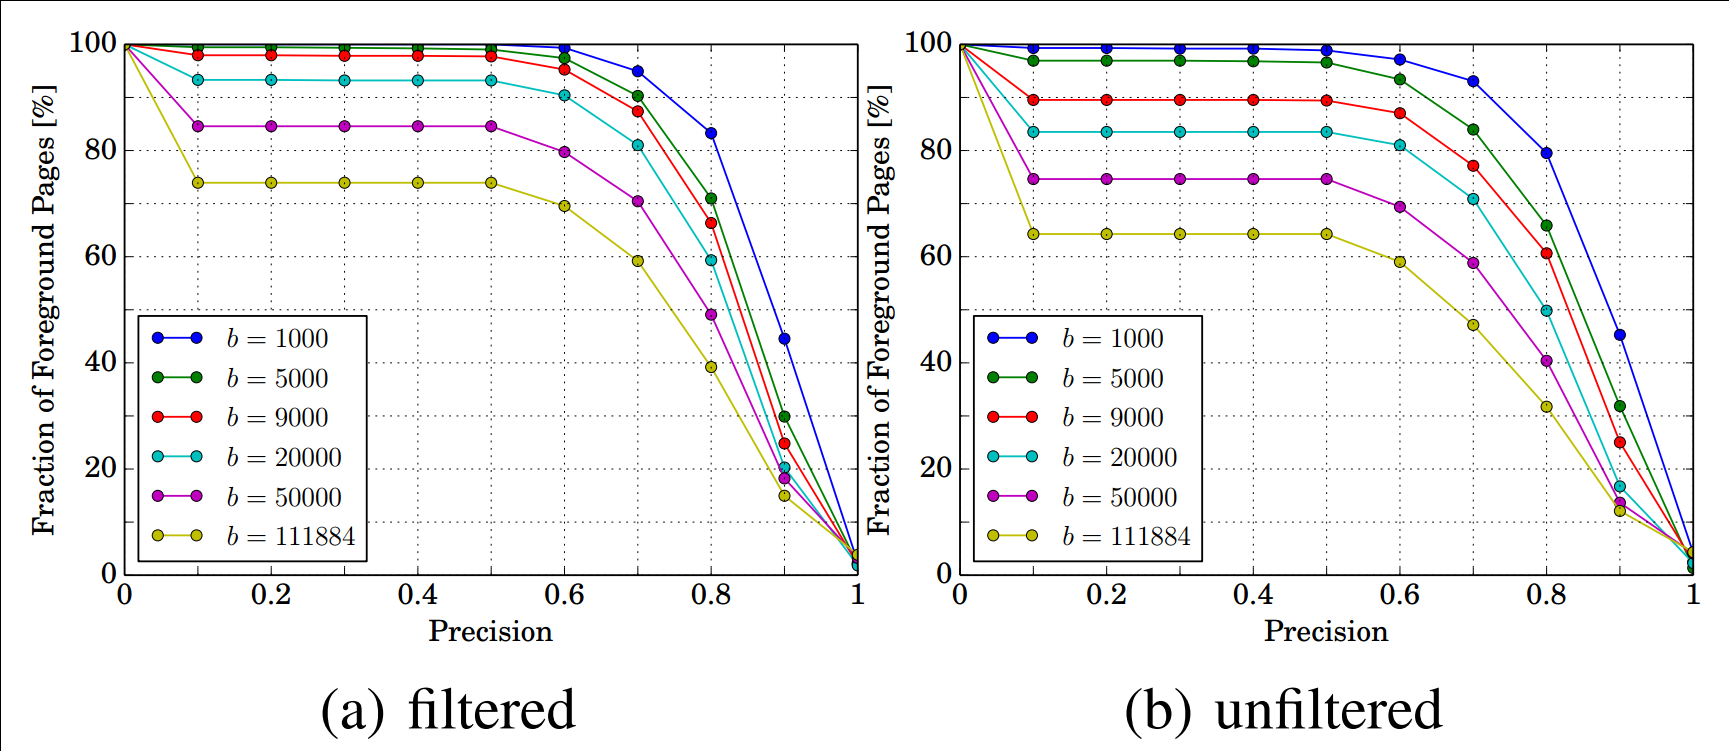
\includegraphics[width=0.8\textwidth,trim={0.4cm 2.5cm 0 0.1cm},clip]{CCDF-Precision}
\newline
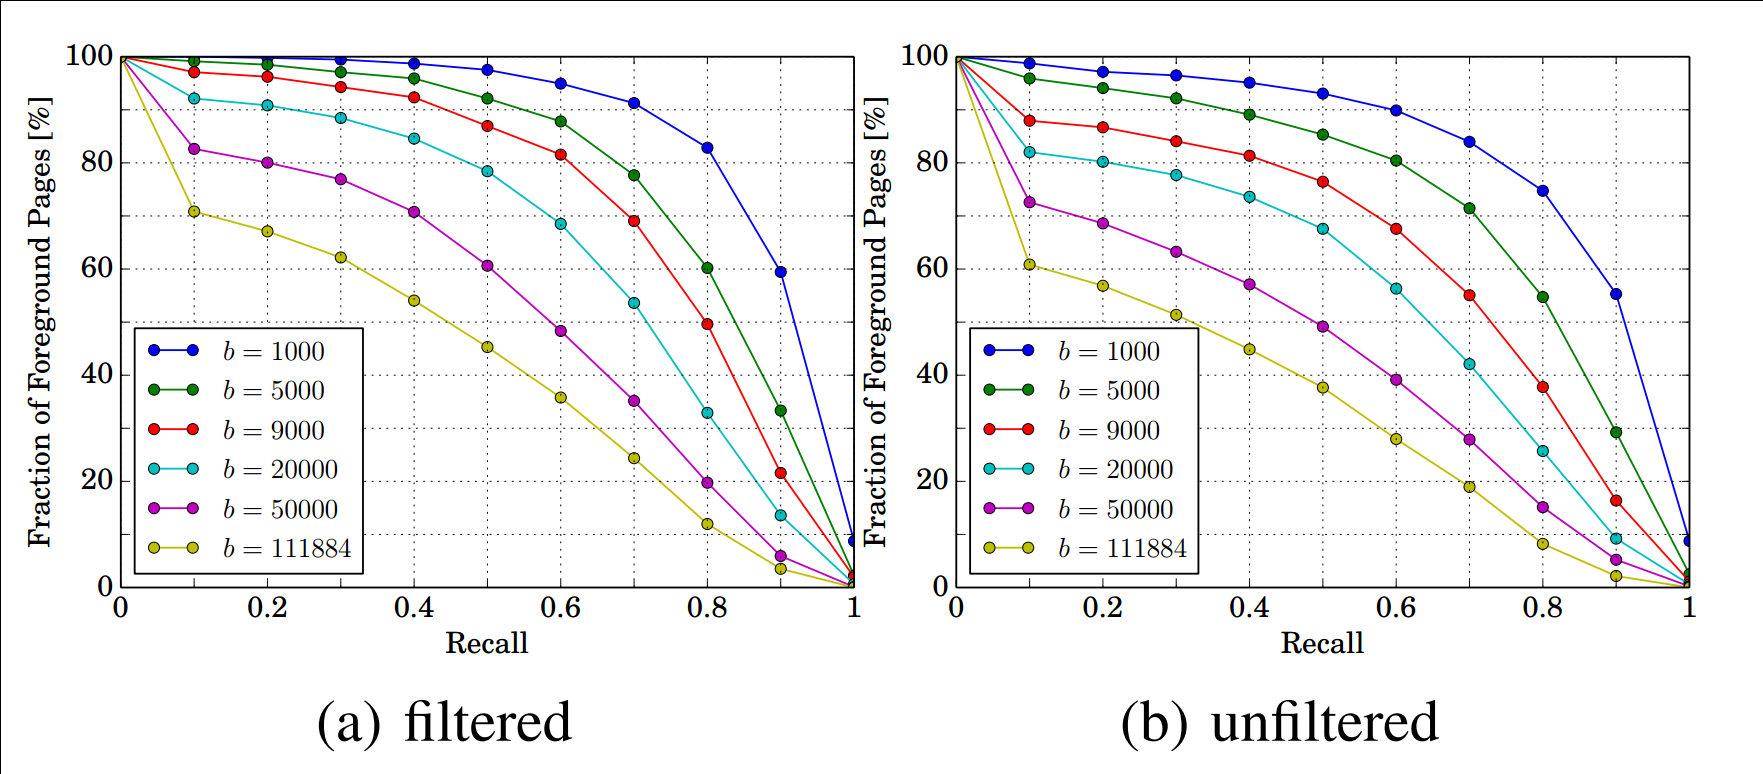
\includegraphics[width=0.8\textwidth,trim={0.1cm 0 0 0.1cm},clip]{CCDF-Recall}
\end{itemize}
\end{frame}

\note[itemize]{
    \item Short answer; No.

    \item Reason for precision / recall over accuracy: If accuracy was used, a
        reject-all strategy would be feasible due to the immense size of web pages in the world.

    \item $b$'s are the number of background pages. Always 1125 foreground pages.

    \item Unfiltered is unchanged background class. Filtered is the foreground page being the only page from a specific web site. The difference is whether web pages that belong to the same website are treated as false positives or not.

    \item Graph type is CCDF, i.e. fraction of $y$'s whose observations are greater than or equal to the value of $x$.

    \item Recall corresponds to the probability that access to a monitored page is detected.

    \item Precision corresponds to the probability that the classifier is actually correct, when it claims a monitored page has been visited.

    \item Which metric is more important depends on the specific use-case.

    \item The general tendency is that larger background set is, the worse the precision and recall.

    \item But as $b = MAX$ (111884) is vanishingly small compared to the entire internet, they conclude that web page fingerprinting is not feasible.
}

\begin{frame}{Evaluation - Results 4 - Web page vs Website}
\begin{itemize}
\item Website fingerprinting feasible versus web page fingerprinting.
\begin{itemize}
\item Closed World results (web page left, website right)
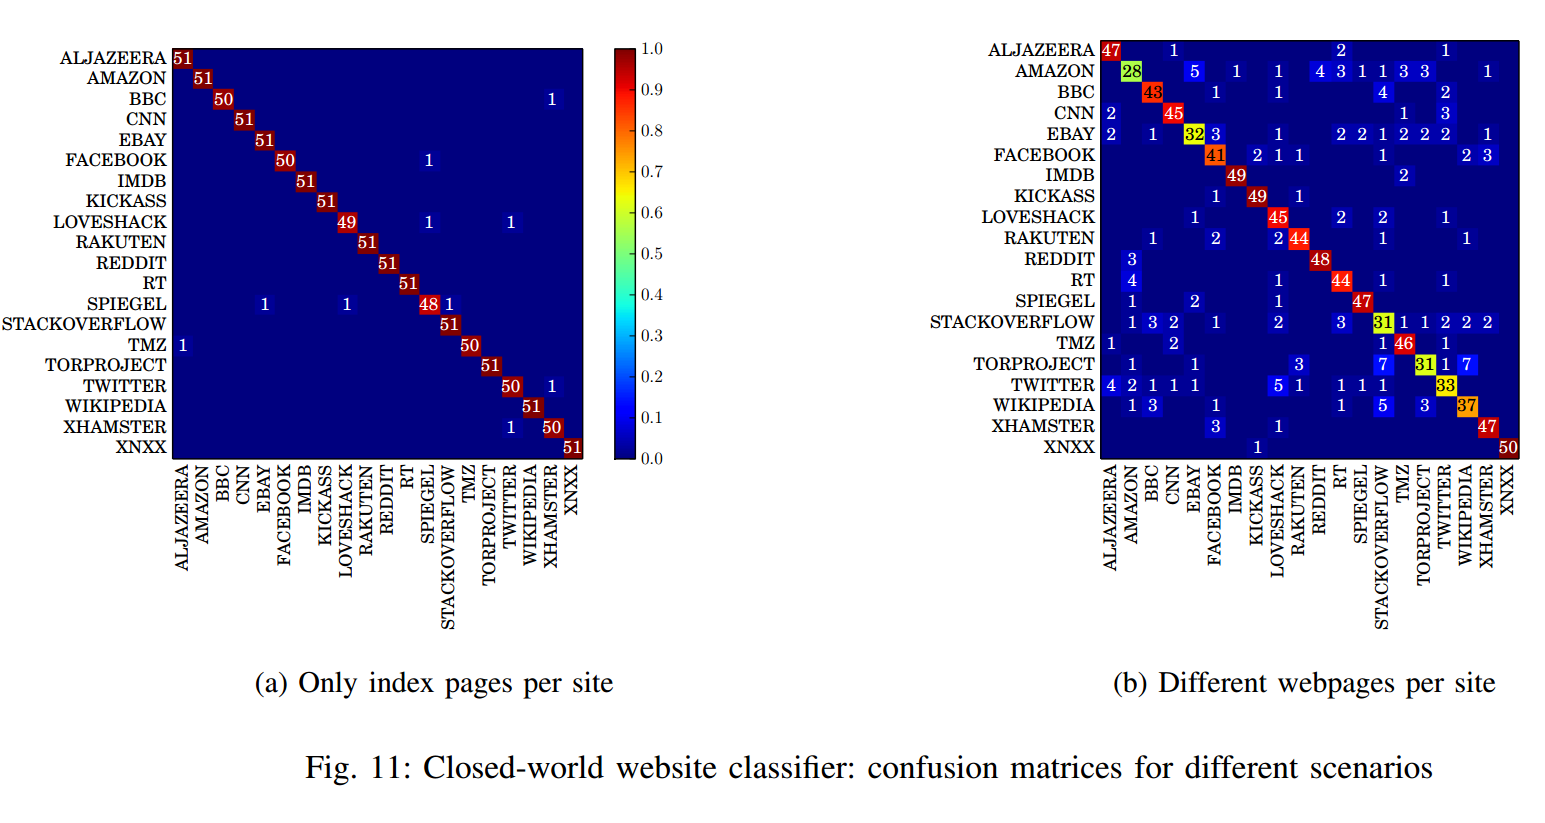
\includegraphics[width=0.8\textwidth,trim={0 5cm 0 0},clip]{Website1}

\item Open World results (website left, web page left)
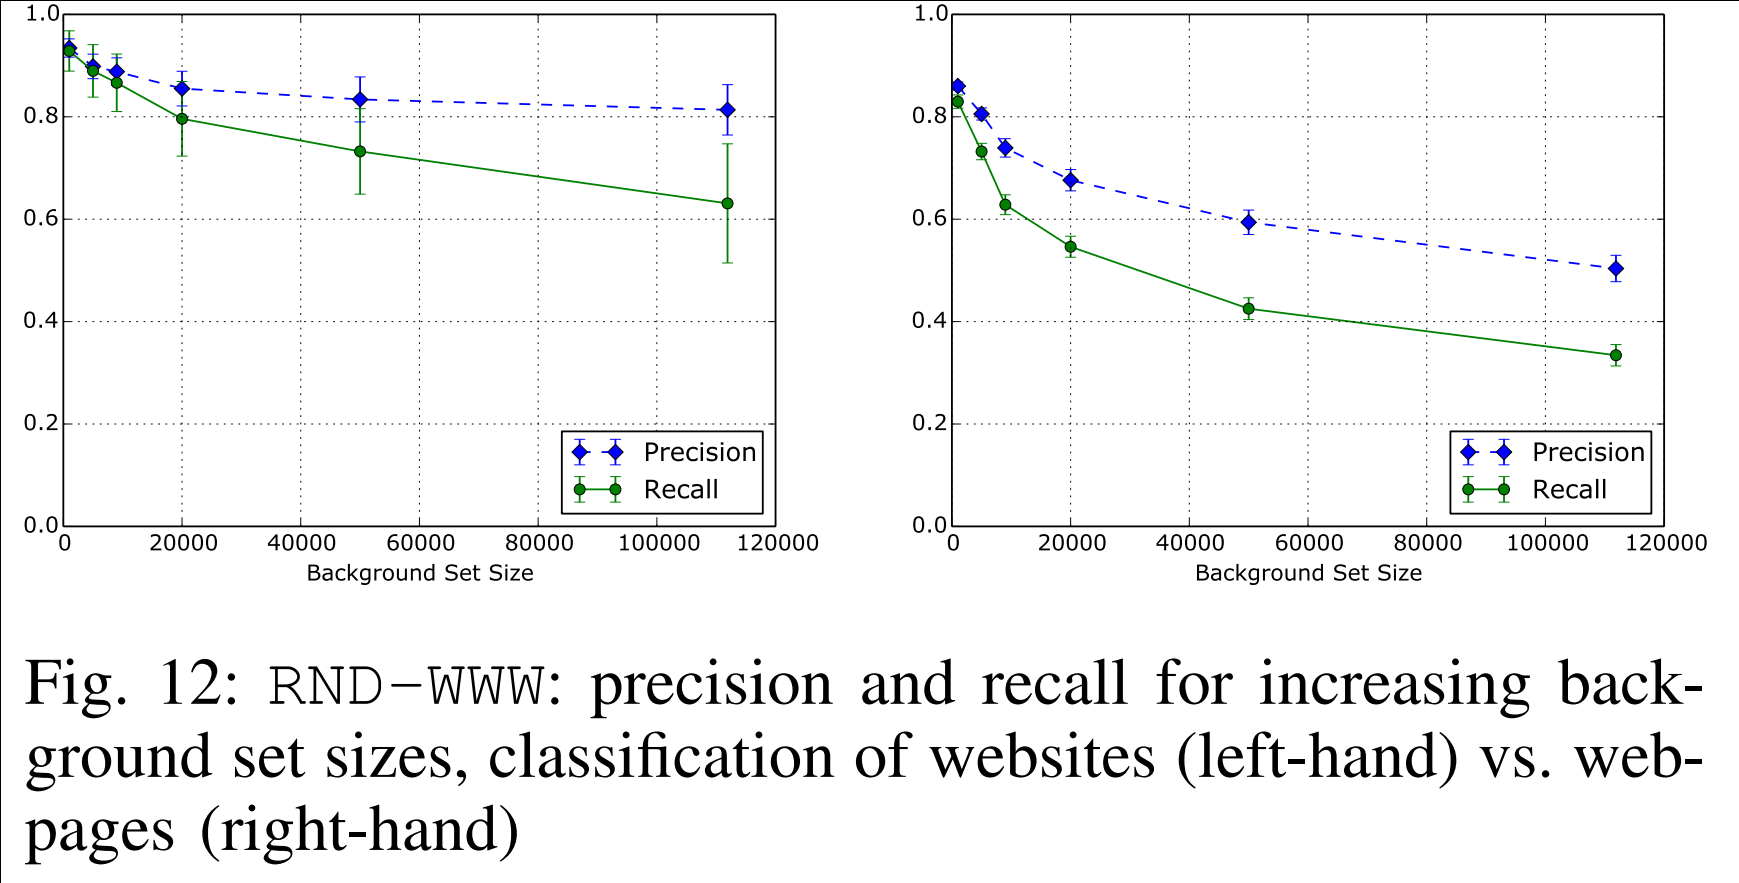
\includegraphics[width=0.8\textwidth,trim={0.1cm 0 0 0.1cm},clip]{Website2}

\end{itemize}
\end{itemize}
\end{frame}

\note[itemize]{
    \item Website fingerprinting for when visits to a website is of interest. \\
        Instead of to specific pages as in the case above.

    \item Fingerprinting web pages yield high number of false positives.

    \item Website fingerprinting less subject to web pages chances. \\
        Which would otherwise decrease accuracy. Because while pages change frequently, the layout of web pages does less so.

    \item Fingerprinting all web pages of a website may be infeasible. \\
        Imagine how many posts there are on Facebook, etc.

    \item Closed World results (99\% vs 82\%), i.e. index page / web page is easier.

    \item Open World results, website finger printing scales better as the number
        of background pages grow, and precision seems to stabilize on a high level.

    \item Point of interest; Web page seemed better in closed world, while website performed better in the more realistic open world scenario.

    \item To increase accuracy in website fingerprinting one should crawl many sites, with few instances, rather than few sites with many instances.
}

\begin{frame}{Paper conclusion}
\begin{itemize}
\item The presented attack is superior in terms of accuracy and computational efficiency.
        When compared to Wang.

\item Further research should use realistic data sets instead of Alexa Top pages.

\item Web page fingerprinting does not scale for any state-of-art attacks. \\
    And thus cannot be used to convict users, but may limit possible suspects.

\item Website fingerprinting is more realistic and effective.

\item Correlating multiple web page loads, may increase accuracy and confidence in the answer.
\end{itemize}
\end{frame}

\note{
    Read the bullet points
}

\section[Project]{Paper versus Project - What can we learn?}
\begin{frame}{Paper versus Project - What can we learn?}
\begin{itemize}
\item Our attack vs Tor
\item Using CUMUL for our Network Bandwidth channel
\item Using CUMULs classification techniques instead of kNN-DTW
\item Using their evaluation methodology / discussion
\end{itemize}
\end{frame}

\note[itemize]{
\item How does our attack do against Tor.

\item How could our in-browser network bandwidth channel be adapted to the methodology used by CUMUL.

\item What can be learned and utilized from their classification techniques in general.

\item How did their evaluation methodology differ;
\begin{itemize}
\item How could we do better?
\item How does the results differ?
\item Is our attack obsolete?
\end{itemize}
}

\begin{frame}{Our attack vs Tor}
\begin{itemize}
\item Normal versus Tor (Subset of retail set) \\
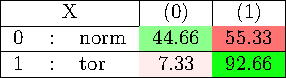
\includegraphics[width=0.5\textwidth]{TorRecall}

\item Accuracy of retail sites via Tor \\
\begin{tabular}{lcc} \hline
        & Ambient   & Load \\ \hline
Tor     & 63.51     & 60.79 \\
Normal  & 97.30     & 96.16 \\ \hline
\end{tabular}
\end{itemize}
\end{frame}

\note{
\begin{itemize}
\item Detecting Tor, our unmodified attack has a 92\% recall for Tor.
    Thereby indicating we will detect visits to pages via Tor.

\item We have 85\% precision for Normal sites.
    So whenever we state a site is not accessed with Tor we are usually right.

\item We can see that our accuracy is adversely affected by Tor. \\
    (10 pages, 30 instances)
    % TODO: Argue why this is the case

\item Thus our attack is significantly worse for detecting Tor pages, but can however be distributed over the internet, as it does not require access to the (encrypted) data flow between the user and Tor. \\
    Which may make it feasible for specific use cases.
\end{itemize}
}

\begin{frame}{Using CUMUL for our Network Bandwidth channel}
% TODO: What can one learn from them w.r.t. browser-based traffic analysis that you performed?
\begin{itemize}
\item Cons: Our Network Bandwidth channel;
\begin{itemize}
\item Is download only - Could be expanded to include upload too
\item Is rather noisy
\item Has low sample rate
\end{itemize}
\item Pros:
\begin{itemize}
\item Can be distributed easily
\end{itemize}
% TODO: More

\end{itemize}
\end{frame}

\note{
\begin{itemize}
\item Apply the entire methodology of CUMUL to our Network Bandwidth Channel
\begin{itemize}
\item We have much lower resolution
\item We will thus have lower accuracy
\item Attack can be distributed globally easily
% TODO: More
\end{itemize}

\end{itemize}
}

\begin{frame}{Using CUMULs classification techniques instead of kNN-DTW}
\begin{itemize}
\item Resampling
\item Feature detecting (alike Wang et al.)
\item Filtering outliers
\item Using SVMs
\item Web page versus website profiling
\end{itemize}
\end{frame}

\note{
\begin{itemize}
\item Resampling: We could resample our data, and acquire a similar accuracy / computational complexity trade-off.

\item Feature detection: Instead of just resampling, we could have done feature detection on our readings, and then process features rather than the entire data set. This would likely improve both accuracy and computational complexity.

\item Filtering outliers:
\begin{itemize}
\item We used $x$ standard derivations
\item They use the 'interquartile range';
\[
    Q_{1} - 1.5(Q_{3} - Q_{1}) < I < Q_{3} + 1.5(Q_{3} - Q_{1})
\]
\end{itemize}

\item Using SVMs: This paper, and the paper by Clark utilized SVMs to achieve great accuracy, and very good rejection rates for unknown pages, as in the open world scenario.

\item Utilizing website profiling: Would be very useful with our ambient readings, and correlation of multiple readings.
\begin{itemize}
\item The user usually clicks around on the same website for a while
\item Thus multiple web pages of that site is visited
\item The effect on correlating readings in this case
\end{itemize}

\end{itemize}
}

\begin{frame}{Evaluation / Discussion}
\begin{itemize}
\item Closed- versus Open world testing
\item Testing data set
\item Degradation of accuracy over time (Referenced paper says):
\begin{itemize}
\item 40\% decrease in less than 10 days
\item almost 0\% accuracy in 90 days
\end{itemize}
Both are for the Alexa Global Top 100.
\item Comparison of results
\end{itemize}
\end{frame}

\note{
\begin{itemize}
\item We only did closed world testing, thus we cannot relate our data to the paper with regards to open world. \\
    And similarly we cannot easily state how well our attack would do in a realistic setting.
\begin{itemize}
\item We only did closed
\item Scale of the attacks
\end{itemize}

\item We tested our data sets against Alexa500 and retail set mainly. \\
    The retail set made good sense for our attack scenario, but we take the point of the work.

\item Degradation of accuracy over time; This challenges our idea of incrementally updating the reference set.

\item We can see that our accuracy is worse with regards to Tor, and we speculate this is the case outside of Tor too. \\
    We do however not reject the attack completely, due to its advantages, namely that it can be distributed massively over the internet, but rather conclude that the attack needs further work to improve its accuracy and computational complexity.
\end{itemize}
}

% XXX: Defenses (from related work)
% Padding
% Random noise / Cover traffic
% Clustered signatures
% Undeterministic signatures by changing pipelining or order of objects downloaded

\end{document}

